Bedeutungen:\\
\begin{tabular}{l l}
$terrorv(x)$ & $x$ ist eine terroristische Vereinigung\\
$terror(x)$ & $x$ ist ein Terrorist\\
$org(x)$ & $x$ ist eine Organisation\\
$mitgl(x,y)$ & $x$ ist Mitglied in Organisation $y$\\
$anf(x,y)$ & $x$ ist Anführer der Organisation $y$\\
$verkauf(x,y,z)$ & $x$ hat $y$ an $z$ verkauft\\
$waffe(x)$ & $x$ ist eine Waffe\\
$strafbar(x)$ & $x$ macht sich strafbar\\
$auto(x)$ & $x$ ist ein Auto
\end{tabular}
\paragraph*{Teil a}
\begin{itemize}
\item $\forall x\; \forall y\;(anf(x,y) \wedge terror(x) \to terrorv(y) )$
\item $\forall x\;\forall y\; (mitgl(x,y) \wedge terrorv(y) \to terror(x))$
\item $\exists x\; (anf(x,\text{IS}) \wedge terror(x))$
\item $mitgl(\text{Abul-Hasan Al Muhajir},\text{IS})$
\item $\forall x\; \forall y\; \forall z ( verkauf(x,y,z) \wedge terror(z) \wedge waffe(y) \to strafbar(x))$
\item $verkauf(\text{Omar Abdul Al-Hassan},\text{M16},\text{Abul-Hasan Al Muhajir})$
\item $waffe(\text{M16})$
\item $mitgl(\text{August Meier})$
\item $org(\text{ADAC})$
\item $verkauf(\text{Bernd Müller}, \text{Auto},\text{August Meier})$
\end{itemize}

\paragraph*{Teil b}
Prolog-Programm:
\lstinputlisting[language=Prolog]{../Praktikum/Prolog/aufg7.pl}
\begin{enumerate}[label=(\roman*)]
\item Abfrage, ob Omar Abdul Al-Hassan strafbar:
\begin{lstlisting}[language=Prolog]
?- strafbar("Omar Abdul Al-Hassan").
true.
\end{lstlisting}
\item Abfrage, ob Bernd Müller strafbar:
\begin{lstlisting}[language=Prolog]
?- strafbar("Bernd Müller").
false.
\end{lstlisting}
\end{enumerate}
\paragraph*{Teil c}
Suchbaum:\\
\resizebox{.99\textwidth}{!}{
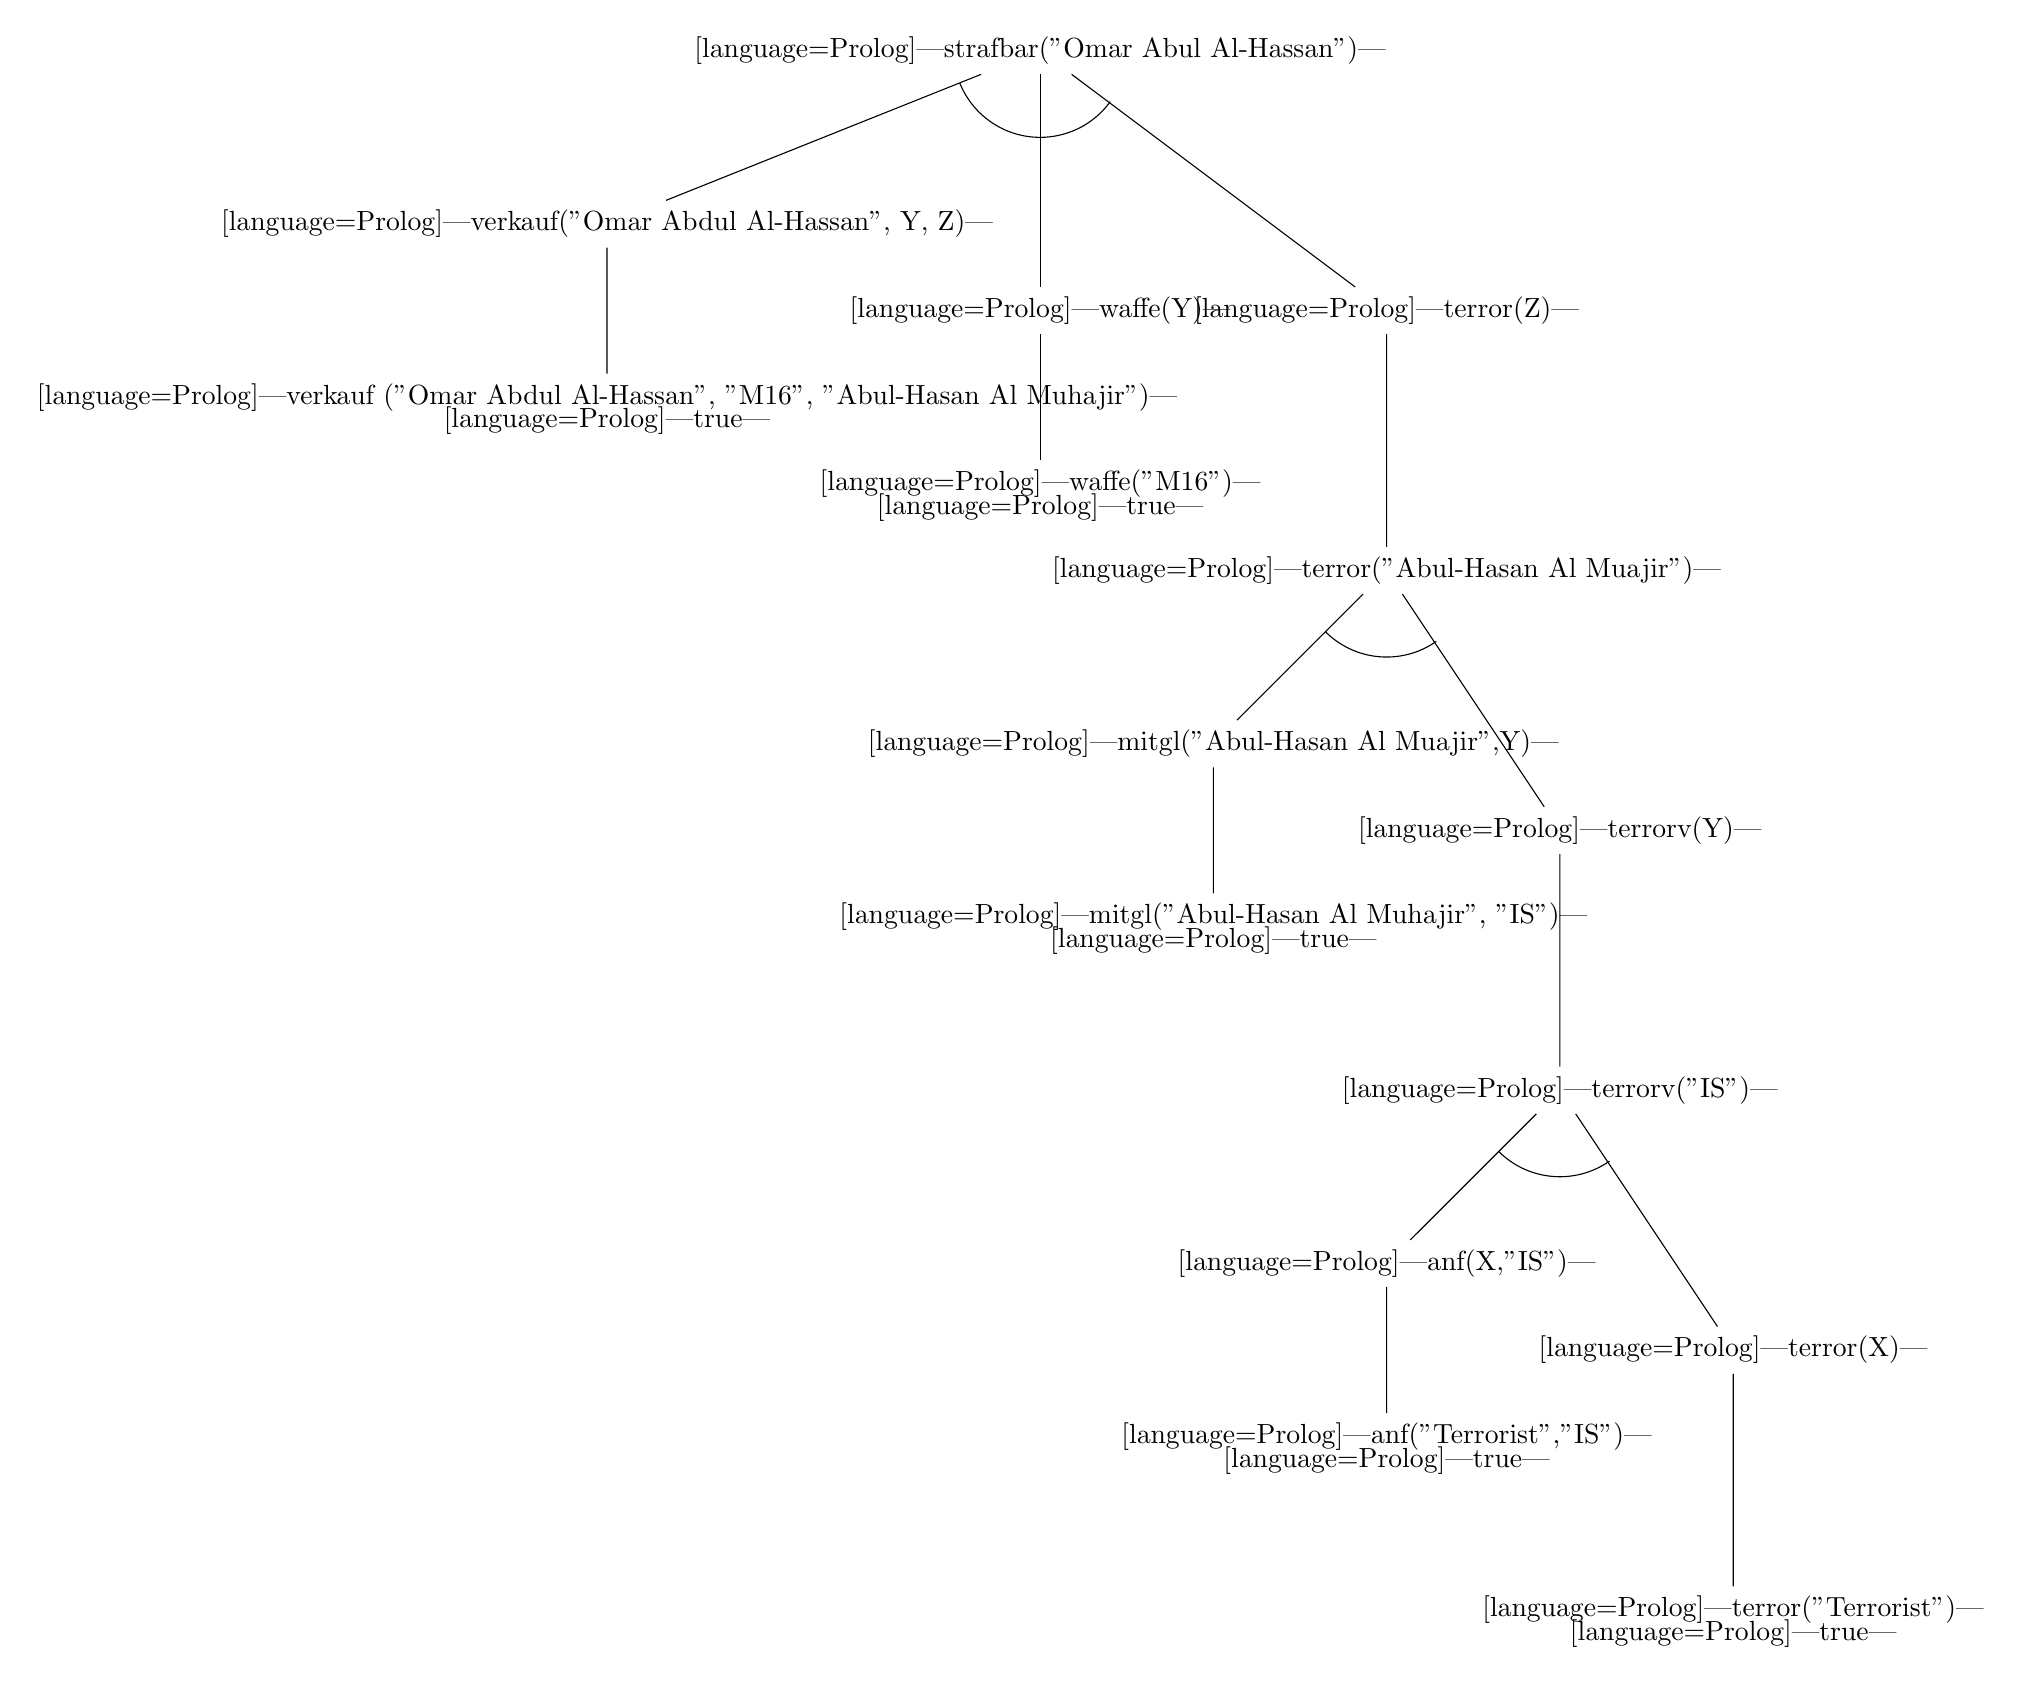
\begin{tikzpicture}[scale=1.1]
\node (v1) at (0,0) {\lstinline[language=Prolog]|strafbar("Omar Abul Al-Hassan")|};
\node (v2) at (-5,-2) {\lstinline[language=Prolog]|verkauf("Omar Abdul Al-Hassan", Y, Z)|};
\node (v4) at (0,-3) {\lstinline[language=Prolog]|waffe(Y)|};
\node (v6) at (4,-3) {\lstinline[language=Prolog]|terror(Z)|};
\node (v3) at (-5,-4) {\lstinline[language=Prolog]|verkauf ("Omar Abdul Al-Hassan", "M16", "Abul-Hasan Al Muhajir")|} (v3) node[below]{\lstinline[language=Prolog]|true|};
\draw (v1) -- (v2) -- (v3);
\node (v5) at (0,-5) {\lstinline[language=Prolog]|waffe("M16")|} (v5) node[below]{\lstinline[language=Prolog]|true|};
\draw (v1) -- (v4) -- (v5);
\node (v7) at (4,-6) {\lstinline[language=Prolog]|terror("Abul-Hasan Al Muajir")|};
\draw (v1) -- (v6) -- (v7);
\node (v8) at (2,-8) {\lstinline[language=Prolog]|mitgl("Abul-Hasan Al Muajir",Y)|};
\node (v10) at (6,-9) {\lstinline[language=Prolog]|terrorv(Y)|};
\node (v9) at (2,-10) {\lstinline[language=Prolog]|mitgl("Abul-Hasan Al Muhajir", "IS")|} (v9) node[below]{\lstinline[language=Prolog]|true|};
\draw (v7) -- (v8) -- (v9);
\node (v11) at (6,-12) {\lstinline[language=Prolog]|terrorv("IS")|};
\node (v12) at (4,-14) {\lstinline[language=Prolog]|anf(X,"IS")|};
\node (v14) at (8,-15) {\lstinline[language=Prolog]|terror(X)|};
\node (v13) at (4,-16) {\lstinline[language=Prolog]|anf("Terrorist","IS")|}(v13) node[below]{\lstinline[language=Prolog]|true|};
\node (v15) at (8,-18) {\lstinline[language=Prolog]|terror("Terrorist")|}(v15) node[below]{\lstinline[language=Prolog]|true|};
\draw (v7) -- (v10) -- (v11) -- (v12) -- (v13);
\draw (v11) -- (v14) -- (v15);
\def\xa{-36};
\def\ra{1cm};
\draw[shift=(\xa : \ra)] (0,0) arc (\xa:-158:\ra);
\def\xb{-55};
\def\rb{1cm};
\draw[shift=(\xb : \rb)] (4,-6) arc (\xb:-135:\rb);
\def\xc{-55};
\def\rc{1cm};
\draw[shift=(\xc : \rc)] (6,-12) arc (\xc:-135:\rc);
\end{tikzpicture}
}